\documentclass[a4paper,english,12pt]{article}
\usepackage{%
	amsfonts,%
	amsmath,%	
	amssymb,%
	amsthm,%
	algorithm,%
	babel,%
	bbm,%
	etex,%
	%biblatex,%
	caption,%
	centernot,%
	color,%
	dsfont,%
	enumerate,%
	epsfig,%
	epstopdf,%
	geometry,%
	graphicx,%
	hyperref,%
	latexsym,%
	mathtools,%
	multicol,%
	pgf,%
	pgfplots,%
	pgfplotstable,%
	pgfpages,%
	proof,%
	psfrag,%
	subfigure,%	
	tikz,%
	ulem,%
	url%
}	
\usepackage[noend]{algpseudocode}
\usepackage[mathscr]{eucal}
\usepgflibrary{shapes}
\usetikzlibrary{%
  	arrows,%
	backgrounds,%
	chains,%
	decorations.pathmorphing,% /pgf/decoration/random steps | erste Graphik
	decorations.text,%
	matrix,%
  	positioning,% wg. " of "
  	fit,%
	patterns,%
  	petri,%
	plotmarks,%
  	scopes,%
	shadows,%
  	shapes.misc,% wg. rounded rectangle
  	shapes.arrows,%
	shapes.callouts,%
  	shapes%
}

\theoremstyle{plain}
\newtheorem{thm}{Theorem}[section]
\newtheorem{lem}[thm]{Lemma}
\newtheorem{prop}[thm]{Proposition}
\newtheorem{cor}[thm]{Corollary}

\theoremstyle{definition}
\newtheorem{defn}[thm]{Definition}
\newtheorem{conj}[thm]{Conjecture}
\newtheorem{exmp}[thm]{Example}
\newtheorem{assum}[thm]{Assumptions}
\newtheorem{axiom}[thm]{Axiom}

\theoremstyle{remark}
\newtheorem{rem}{Remark}
\newtheorem{note}{Note}
\newtheorem{fact}{Fact}

\newcommand{\norm}[1]{\left\lVert#1\right\rVert}
\newcommand{\indep}{\!\perp\!\!\!\perp}
\DeclarePairedDelimiter\abs{\lvert}{\rvert}%
\newcommand\numberthis{\addtocounter{equation}{1}\tag{\theequation}}
\newcommand{\tr}{\operatorname{tr}}
\newcommand{\R}{\mathbb{R}}
\newcommand{\N}{\mathbb{N}}
\newcommand{\E}{\mathbb{E}}
\newcommand{\Z}{\mathbb{Z}}
\newcommand{\B}{\mathscr{B}}
\newcommand{\C}{\mathcal{C}}
\newcommand{\T}{\mathscr{T}}
\newcommand{\F}{\mathcal{F}}
\newcommand{\G}{\mathcal{G}}
%\newcommand{\ba}{\begin{align*}}
%\newcommand{\ea}{\end{align*}}
\DeclareMathOperator*{\argmax}{arg\,max}
\renewcommand{\qedsymbol}{$\blacksquare$}
\makeatletter
\def\BState{\State\hskip-\ALG@thistlm}
\makeatother

\makeatletter
\def\th@plain{%
  \thm@notefont{}% same as heading font
  \itshape % body font
}
\def\th@definition{%
  \thm@notefont{}% same as heading font
  \normalfont % body font
}
\makeatother
\date{}

\title{Lecture 10: Signal Detection in Discrete Time}
\date{12 February 2016}


\begin{document}
\maketitle

\section{Introduction}
In this lecture we apply the theory of hypothesis-testing to detect or discern signals corrupted by noise. We try to build a model which will perform this task of detecting signals embedded in noise. The most common application of this theory is in communication receivers. Some other applications are in the field of radar and sonar receivers, radio astronomy, experimental physics, etc.
\section{Models and Detector Structures}
The basic physical model we consider is that of an observed continuous-time waveform that consists of one of the two possible signals embedded in noise.
\par Consider having \textit{n} samples of the waveform being observed and let the signal be denoted by an \textit{n} length vector $\underline{Y}=(Y_{1},...,Y_{n})^{T}$. Similarly, let $\underline{N}=(N_{1},...,N_{n})^{T}$ be a vector of noise samples, and $\underline{S}_{0}=(S_{01},...,S_{0n})^{T}$ and $\underline{S}_{1}=(S_{11},...,S_{1n})^{T}$ be the vectors of samples from the two possible signals.
\par This problem can be modelled statistically by the following hypothesis for the observation space ($\Gamma$,$\mathcal{G}$)=$({\rm I\!R}^{\text{n}},\mathcal{B}^{\text{n}})$:
\begin{equation}
\begin{split}
\label{hypothesis}
&H_{0}: Y_{k} = N_{k}+S_{0k}, \hspace{10pt}k=1,2,...,n\\
\text{versus}\hspace{10pt}&
\\&H_{1}: Y_{k} = N_{k}+S_{1k}, \hspace{10pt}k=1,2,...,n.	
\end{split}
\end{equation}
Depending on the nature of the signals $\underline{S}_{0}$ and $\underline{S}_{1}$, we can have three cases: 
\begin{enumerate}
\item $\underline{S}_{0}$ and $\underline{S}_{1}$ are completely known (i.e., deterministic).
\item $\underline{S}_{0}$ and $\underline{S}_{1}$ are partially known except for a set of unknown (possibly random) parameters.
\item $\underline{S}_{0}$ and $\underline{S}_{1}$ are completely unknown and thus specified only by their probability distribution.
\end{enumerate}
\begin{assum}
$\underline{S}_{0}=\underline{0}$ (an all zero vector) and $\underline{S}_{1}=\underline{S}$.
\end{assum}
\begin{assum}
The noise is independent of the signal i.e. at each time instant k, the sample is corrupted by independent noise, and the noise distribution is determined by density $p_{N}$ on ${\rm I\!R}^{n}$.
\end{assum}
With the above discussed framework and assumptions made, the likelihood ratio for (\ref{hypothesis}) can be computed if the statistic of $\underline{S}_{j}$ for $j=0,1$ is known. Given that $\underline{S}_{j}$=$\underline{s}_{j}$ $\in {\rm I\!R}^{\textbf{n}}$, the conditional density of $\underline{Y}$ (under $H_{j}$) is given by 
\begin{equation}
\label{cond_density}
p_{\underline{N}}(\underline{y}-\underline{s}_{j}),\hspace{10pt}\underline{y}\in{\rm I\!R}^{\text{n}}.
\end{equation}
From (\ref{cond_density}) we see that the density of $\underline{Y}$ under $H_{j}$ is given by
\begin{equation}
\label{density}
p_{j}(\underline{y})=E\{p_{\underline{N}}(\underline{y}-\underline{S}_{j})\},\hspace{10pt}\underline{y}\in{\rm I\!R}^{\text{n}},
\end{equation}
where $E\{.\}$ the expectation is with respect to signal $\underline{S}_{j}$. The general expression of the likelihood ratio for (\ref{hypothesis}) is given by
\begin{equation}
\label{L(y)}
L(\underline{y})=\frac{E\{p_{\underline{N}}(\underline{y}-\underline{S}_{1})\}}{E\{p_{\underline{N}}(\underline{y}-\underline{S}_{0})\}},\hspace{10pt}\underline{y}\in{\rm I\!R}^{\text{n}}.
\end{equation}
\subsection{Case I: Detection of Deterministic Signals in Independent Noise}
As discussed earlier, here the two signals $\underline{S}_{0}$ and $\underline{S}_{1}$ are completely known or deterministic. In the field of communication, this is known as the $coherent\ detection$ problem. Here, $L(\underline{y})$ of (\ref{L(y)}) becomes
\begin{eqnarray}
\label{L(y)_coherent_initial}
L (\underline{y})&=&\frac{p_{\underline{N}}(\underline{y}-\underline{s}_{1})}{p_{\underline{N}}(\underline{y}-\underline{s}_{0})},\nonumber\\
&=&\frac{p_{\underline{N}}(y_{1}-s_{11},y_{2}-s_{12},...,y_{n}-s_{1n})} {p_{\underline{N}}(y_{1}-s_{01},y_{2}-s_{12},...,y_{n}-s_{0n})},
\end{eqnarray}
since the noise samples $N_{1},N_{2},...,N_{n}$ are statistically independent (by assumption). So we have
\begin{equation}
p_{\underline{N}}(\underline{y})= \prod_{k=1}^{n}   p_{N_{k}}(y_{k}),
\end{equation}
where $p_{N_{k}}$ is the marginal density of $N_{k}$. So, $L({\underline{y}})$ of (\ref{L(y)_coherent_initial}) becomes  
\begin{equation}
\label{L(y)_Coherent}
L_(\underline{y})= \prod_{k=1}^{n}\frac{p_{N_{k}}(y_{k}-s_{1k})}{p_{N_{k}}(y_{k}-s_{0k})}.
\end{equation}
Comparing this $L(\underline{y})$ to a threshold $\tau$ gives us the decision rule
\begin{equation}
\tilde\delta_{o}(\underline{y})=\begin{cases} 
1 &>\\
\gamma \hspace{20pt}\text{if } L(\underline{y}) &= \hspace{10pt}\tau.\\
0 &<
\end{cases}
\end{equation}
\begin{exmp}[Coherent Detection in i.i.d Gaussian Noise]
\label{caseI}
Suppose that the noise samples $N_{1},...,N_{n}$ are independent and identically distributed (i.i.d.) with marginal distribution $\mathcal{N}(0,\sigma^2)$. Without any loss of generality, assuming $\underline{s}_{0}= \underline{0}$ (all zero vector) and $\underline{s}_{1}= \underline{s}$, $L(\underline{y})$ of (\ref{L(y)_Coherent}) can be written as
\begin{equation}
L(\underline{y})=\prod_{k=1}^{n}\exp\left(-\frac{(y_{k}-s_{k})^2}{2\sigma^2}+\frac{(y_{k})^2}{2\sigma^2}\right).
\end{equation}
Taking log on both sides, log $L(\underline{y})$ can be expressed as
\begin{eqnarray}
\log L(\underline{y})
  &=& \sum_{k=1}^{n}-\frac{(y_{k}-s_{k})^2}{2\sigma^2}+\frac{(y_{k})^2}{2\sigma^2}, \nonumber\\
  &=& \sum_{k=1}^{n}\frac{-(y_{k}^2+s_{k}^2-2y_{k}s_{k})+y_{k}^2}{2\sigma^2}, \nonumber\\
  &=& \sum_{k=1}^{n}\frac{2 y_{k} s_{k}-s_{k}^2 }{2\sigma^2}, \nonumber\\
  &=& \frac {1}{\sigma^2}\sum_{k=1}^{n}s_{k}(y_{k}-s_{k}/2). 
\end{eqnarray}
Thus the decision rule becomes
\begin{equation}
{\tilde\delta_{o}(\underline{y})}= \begin{cases} 
1 &>\\
\gamma \hspace{20pt}\text{if }\sum_{k=1}^{n}s_{k}(y_{k}-s_{k}/2)&=\hspace{10pt}\sigma^2\log\tau,\\
0 &<
\end{cases}
\end{equation}
or equivalently
\begin{equation}
{\tilde\delta_{o}(\underline{y})}= \begin{cases} 
1 &>\\
\gamma \hspace{20pt}\text{if }\sum_{k=1}^{n}s_{k}y_{k}&=\hspace{10pt}\tau',\\
0 &<
\end{cases}
\end{equation}
where $\tau'\triangleq\sigma^2\log\tau+\frac{1}{2}\sum_{k=1}^{n}s_{k}^2$. This detector structure is depicted in Fig. \ref{fig:Fig1}.
\begin{figure}[h]
\centering
\captionsetup{justification=centering}
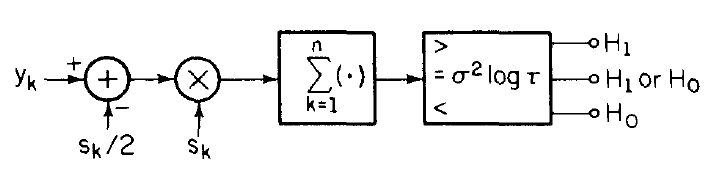
\includegraphics[width=0.8\linewidth]{Figures/lec10Fig1}
\caption{Optimum detector for coherent signals i.i.d Gaussian noise}
\caption*{\footnotesize(\textit{Source: H. Vincent Poor, An Introduction to Signal Detection and Estimation(Second Edition), Figure	 III.B.2(a)})}
\label{fig:Fig1}
\end{figure}
\par This system centers the observation by subtracting $s_{k}/2$ from each $y_{k}$. It correlates the centered data with the known signal and compares the output of this correlation with a threshold. It can be viewed as a system that inputs the observation sequence $(y_{1}, y_{2}....,y_{n})$ to a linear digital filter and then samples the output at time n for comparison with a threshold. Such a structure is known as a {\it matched filter}.
\end{exmp}
\begin{exmp}[Coherent Detection in i.i.d Laplacian Noise]
Suppose, as in Example \ref{caseI}, that the noise samples $N_{1},...,N_{n}$ are i.i.d but with Laplacian marginal probability density
\begin{equation}
\label{density_Laplacian}
p_{N_{k}}(y_{k}) = \frac{\alpha}{2} e^{-\alpha |y_{k}|},\hspace{10pt}y_{k}\in {\rm I\!R} ,
\end{equation}
where $\alpha>0$ is a scale parameter of the density. This model is sometimes used to represent the behavior of impulsive or burst noise in communication receivers.
\par The function $\log L_{k}(y_{k})$ for (\ref{density_Laplacian}) is given by $\log L_{k}(y_{k})=\alpha(|y_{k}|-|y_{k}-s_{k}|)$, which can be written as
\begin{equation}
\log L_{k}(y_{k})=\begin{cases}
-\alpha|s_{k}|&\text{if } \text{sgn } (s_{k})y_{k}\leq0\\
\alpha|2y_{k}-s_{k}|&\text{if }0<\text{sgn }(s_{k})y_{k}<|s_{k}|\\
+\alpha|s_{k}|&\text{if }\text{sgn }(s_{k})y_{k}\geq|s_{k}|,
\end{cases}
\end{equation}
where $sgn$ denotes the signum function
\begin{equation}
\text{sgn }(x)=\begin{cases}
+1&\text{if }x>0\\
0&\text{if }x=0\\
-1&\text{if }x<0.
\end{cases}
\end{equation}
\begin{figure}[h]
\centering
\captionsetup{justification=centering}
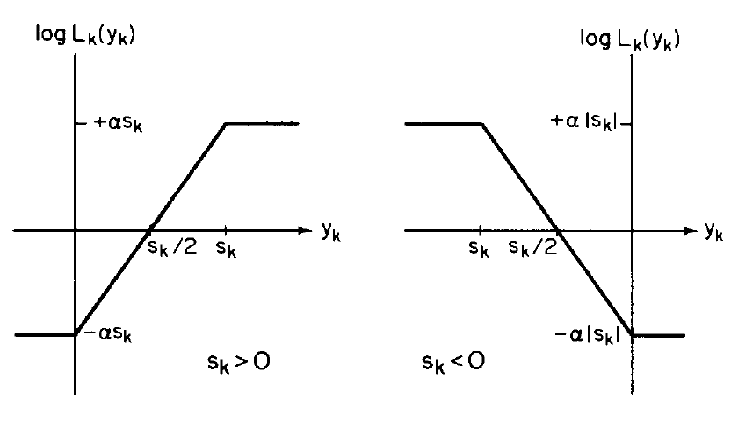
\includegraphics[width=0.8\linewidth]{Figures/lec10Fig2}
\caption{Per-sample log-likelihood ratio for coherent detection in Laplacian Noise}
\caption*{\footnotesize(\textit{Source: H. Vincent Poor, An Introduction to Signal Detection and Estimation(Second Edition), Figure	 III.B.3})}
\label{fig:Fig2}
\end{figure}
\par This function $\log L_{k}(y_{k})$ for both cases ($s_{k}>0\ and\ s_{k}<0$) is depicted in Fig. \ref{fig:Fig2}. By inspection of these figures the decision rule can be written as
\begin{equation}
\tilde\delta_{o}(\underline{y})=\begin{cases}
1,&>\\
\gamma,\hspace{10pt}\text{if }\sum_{k=1}^{n}\text{sgn }(s_{k})l_{k}(y_{k}-s_{k}/2)&=\tau,\\
0,&<
\end{cases}
\end{equation}
where the function $l_{k}$ is given by
\begin{equation}
l_{k}(x)=\begin{cases}
-|s_{k}|/2,&\text{if }x\leq-|s_{k}|/2,\\
x,&\text{if }-|s_{k}|/2<x<|s_{k}|/2,\\
+|s_{k}|/2,&\text{if }x\geq+|s_{k}|/2.
\end{cases}
\end{equation}
\par Such a function is known as a $soft\ limiter/amplifier\ limiter$. The structure for such a model is depicted in Fig. \ref{fig:Fig3}.
\begin{figure}[h]
\centering
\captionsetup{justification=centering}
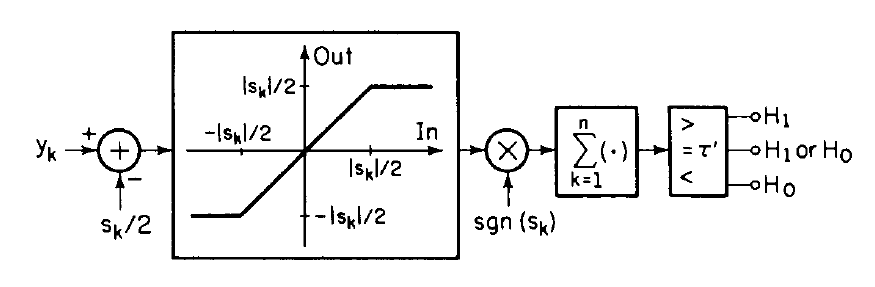
\includegraphics[width=0.8\linewidth]{Figures/lec10Fig3}
\caption{Optimum detector for coherent signals in Laplacian Noise}
\caption*{\footnotesize(\textit{Source: H. Vincent Poor, An Introduction to Signal Detection and Estimation(Second Edition), Figure	 III.B.4})}
\label{fig:Fig3}
\end{figure}
\par This detector also centers the observation by subtracting $s_{k}/2$ from each $y_{k}$. Then it soft limits the centered data and then correlates these soft limited observations with the sequence of signal signs. The effect of soft limiting is to reduce the effect of large observations on the sum, thus making the system more tolerant to large noise values.
\end{exmp}
\begin{exmp}[Locally Optimum Detection of Coherent Signals in i.i.d. Noise]
Often in many detection problems the form of the received signals is known but not its amplitude. To model such a problem we consider the composite hypothesis-testing problem given by:
\begin{equation}
\begin{split}
\label{hypothesis_local}
&H_{0}: Y_{k} = N_{k}, \hspace{10pt}k=1,2,...,n\\
\text{versus}\hspace{10pt}&
\\&H_{1}: Y_{k} = N_{k}+\theta{s_{k}}, \hspace{10pt}k=1,2,...,n,\hspace{10pt}\theta>0,
\end{split}
\end{equation}
where $\underline{s}=(s_{1},...,s_{n})^T$ is a known signal, $\underline{N}=(N_{1},...,N_{n})^T$ is a continuous random vector with i.i.d. components and marginal probability density functions $p_{N_{k}}$, and $\theta$ is an unknown signal-strength parameter, i.e. signal $s_{k}$ should have been scaled with unknown amplitude $\theta$, where the distribution is
\begin{eqnarray}
\Lambda_{0}&=&\{0\},\hspace{10pt}\theta=0\nonumber\\
\Lambda_{1}&=&(0,\infty),\hspace{10pt}\theta>0.\nonumber
\end{eqnarray}
For any particular (given) $\theta$, the $L_{\theta}(\underline{y})$ of (\ref{hypothesis_local}) is given by
\begin{equation}
\label{L(y)_theta}
L_{\theta}(\underline{y})=\prod_{k=1}^{n}\frac{p_{N_{k}}(y_{k}-\theta s_{k})}{p_{N_{k}}(y_{k})}.
\end{equation}
The critical region for any $\theta$,
$\Gamma_{\theta}=\{\underline{y}\in{\rm I\!R}^n|L_{\theta}(\underline{y})>\tau\}$ will generally depend on $\theta$. Hence a $uniformly\ most\ powerful$ (UMP) test may not exist. Instead, we can try to find a $locally\ most\ powerful$ (LMP) test. It is in some sense optimal when $\theta$ is very close to 0.
\begin{note}
Suppose that $ \Lambda_{0}=\{\theta_{0}\} $ and $ \Lambda_{1}=(\theta_{0},\infty) $. Given $\alpha\in$ $ (0,1) $ an $ \alpha $-level LMP test carries out
\begin{equation}
\max_{\delta} \left(P_{D}^\prime(\delta,\theta_{o})=\frac{\partial}{\partial\theta}P_{D}(\delta,\theta)\hspace{2pt}\Bigg|_{\theta=\theta_{o}} \right),\nonumber
\end{equation}
such that $P_{F}(\delta)\leq\alpha$.
\par Thus, the form of LMP will be
\begin{equation}
\tilde\delta_{lo}(y)=\begin{cases}
1&>\\
\gamma\hspace{10pt}\text{if }\frac{\partial}{\partial\theta}P_{\theta}(y)\hspace{2pt}\big|_{\theta=\theta_{o}}&=\eta.P_{\theta_{o}}(y).\\
0&<
\end{cases}
\end{equation} 
\end{note}
Upon differentiation of (\ref{L(y)_theta}), we have
\begin{eqnarray}
\frac{{\partial}}{\partial\theta}L_{\theta}(\underline{y})\hspace{2pt}|_{\theta=0}&=&\frac{\partial}{\partial\theta}\left(\prod_{k=1}^n\frac{p_{N_{1}}(y_{k}-\theta_{S_{k}})}{p_{N_{1}}(y_{k})}\right)\hspace{2pt}\Bigg|_{\theta=0}\nonumber\\
&=&\left(\prod_{k=1}^n\frac{p_{N_{1}}(y_{k}-\theta_{S_{k}})}{p_{N_{1}}(y_{k})}\right)\left(\sum_{k=1}^{n}\frac{\frac{\partial}{\partial\theta}p_{N_{1}}(y_{k}-\theta_{S_{k}})}{p_{N_{1}}(y_{k}-\theta_{S_{k}})}\right)\Bigg|_{\theta=0}\nonumber\\
&=&\sum_{k=1}^{n}\frac{-s_{k}p_{N_{1}}^\prime(y_{k}-\theta_{S_{k}})}{p_{N_{1}}(y_{k}-\theta_{S_{k}})}\Bigg|_{\theta=0}\nonumber\\
&=&\sum_{k=1}^{n}s_{k}\left(\frac{-p_{N_{1}}^\prime(y_{k})}{p_{N_{1}}(y_{k})}\right)\nonumber\\
&=&\sum_{k=1}^{n}s_{k}g_{lo}(y_{k}),
\end{eqnarray}
\begin{figure}[h]
\centering
\captionsetup{justification=centering}
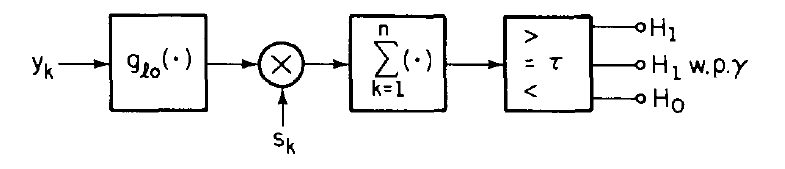
\includegraphics[width=0.8\linewidth]{Figures/lec10Fig4}
\caption{Locally optimum detector structure for coherent signals in i.i.d noise}
\caption*{\footnotesize(\textit{Source: H. Vincent Poor, An Introduction to Signal Detection and Estimation(Second Edition), Figure	 III.B.5})}
\label{fig:Fig4}
\end{figure}\
\begin{figure}[h]
\centering
\captionsetup{justification=centering}
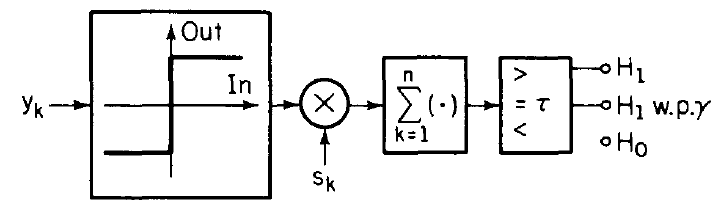
\includegraphics[width=0.8\linewidth]{Figures/lec10Fig5}
\caption{Locally optimum detector for Laplacian noise}
\caption*{\footnotesize(\textit{Source: H. Vincent Poor, An Introduction to Signal Detection and Estimation(Second Edition), Figure	 III.B.6})}
\label{fig:Fig5}
\end{figure}
where $g_{lo}(x)\triangleq-\ p_{N_{1}}^\prime(x)/p_{N_{1}}(x)$, and where $p_{N_{1}}^\prime(x)=dp_{N_{1}}(x)/dx$. This structure is depicted in  Fig. \ref{fig:Fig4}. It consists of the memoryless non-linearity $g_{lo}$ followed by a correlator, a combination known as a $nonlinear\ correlator$.
\par Like the likelihood ratio, the locally optimum nonlinearity $g_{lo}$, shapes the observations to reduce the detrimental effects of the noise as much as is possible. For example, with $\mathcal{N}(0,\sigma^2)$ noise, we have $g_{lo}(x)=x/\sigma^2$, so that  Fig. \ref{fig:Fig4} is simply the correlation detector of Fig.\ref{fig:Fig1}. This must be so; since this detector is UMP, it is also LMP.
\par For Laplacian noise with density (\ref{density_Laplacian}) we have $g_{lo}(x)=\alpha\ $sgn$\ (x)$. The locally optimum detector correlates the signal with the sequences of signs of the observations as depicted in Fig. \ref{fig:Fig5}. The function $g_{lo}(x)$ in this case is known as a $hard\ limiter$.
\end{exmp}
\end{document}